\section{Experiments}

In \S\ref{ssec:synth} we first describe our results on extensive synthetic experiments performed with our model in two conditions:
1) views missing at random for each dataset,
and 2) datasets with systematically missing views (missing not at random).
In \S\ref{ssec:real} we evaluate the prediction error of our model when modeling multiple multi-view real datasets.

%%%%%%%%%%%%%%%%%%%%%%%%%%%
%% SYNTHETIC EXPERIMENTS %%
%%%%%%%%%%%%%%%%%%%%%%%%%%%
\subsection{Synthetic Experiments}
\label{ssec:synth}
\begin{figure}[htb]
\centering
\begin{subfigure}{.49\textwidth}
	\centering
        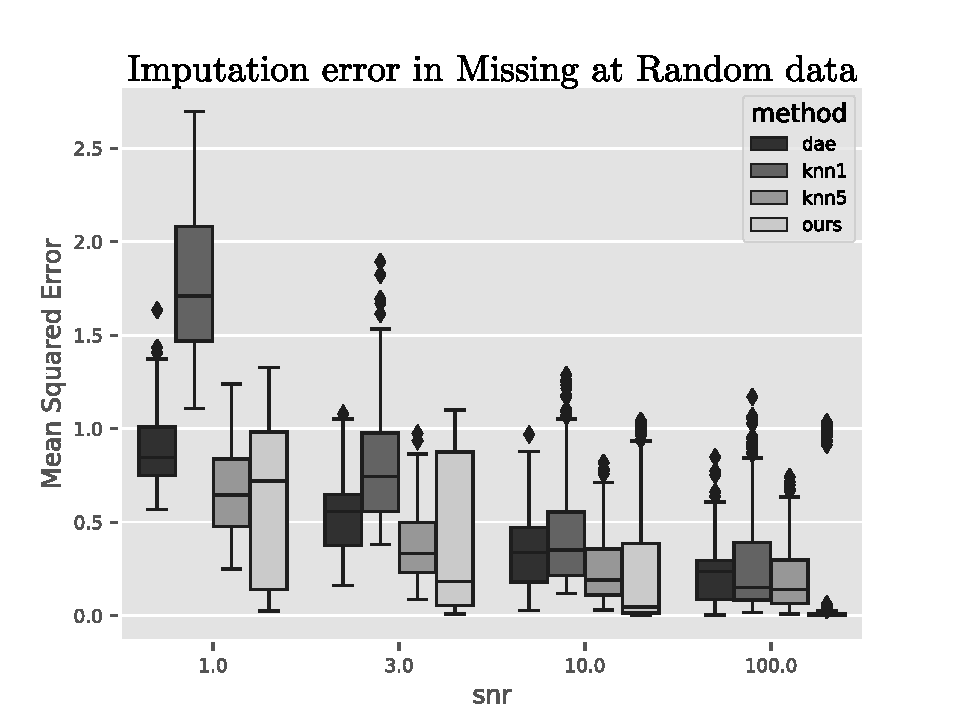
\includegraphics[width=\textwidth]{./tex/fig/mar_imput_err_boxplot.pdf}
        \caption{Missing at random}
        \label{fig:synthetic_benchmark_mar_box}
\end{subfigure}%
\hfill
\begin{subfigure}{.49\textwidth}
	\centering
        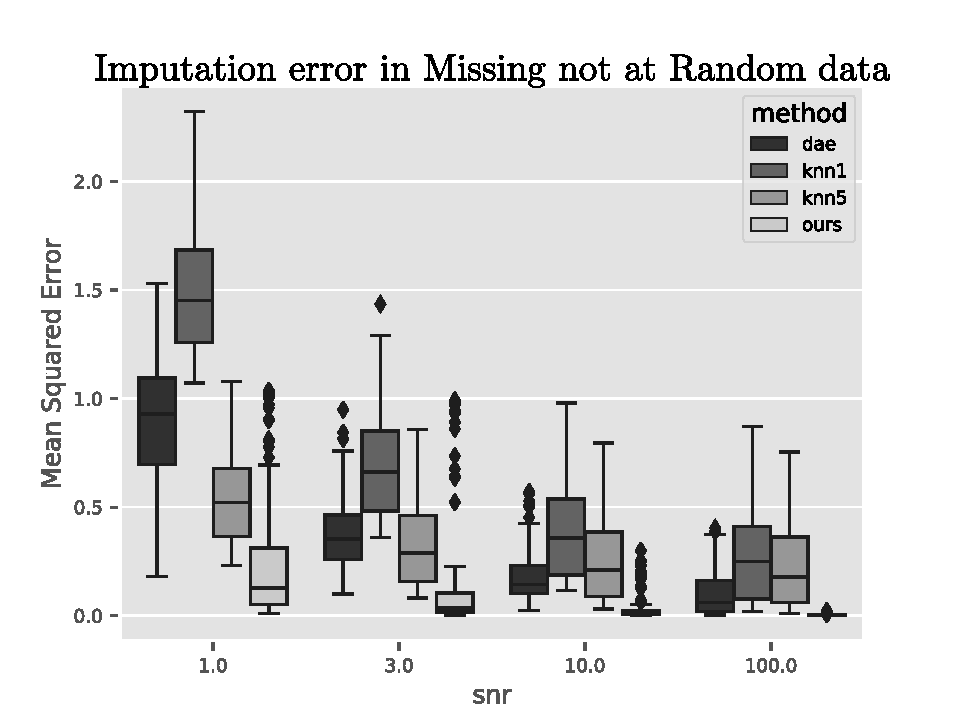
\includegraphics[width=\textwidth]{./tex/fig/mnar_imput_err_boxplot.pdf}
        \caption{Missing not at random}
        \label{fig:synthetic_benchmark_mnar_box}
\end{subfigure}
\caption{
Mean Squared Error of imputation in synthetic datasets. Effect of signal-to-noise ratio (\snr) is shown.
}
\label{fig:synthetic_benchmark_box}
\end{figure}

\begin{figure}[htb]
\centering
\begin{subfigure}{.49\textwidth}
	\centering
        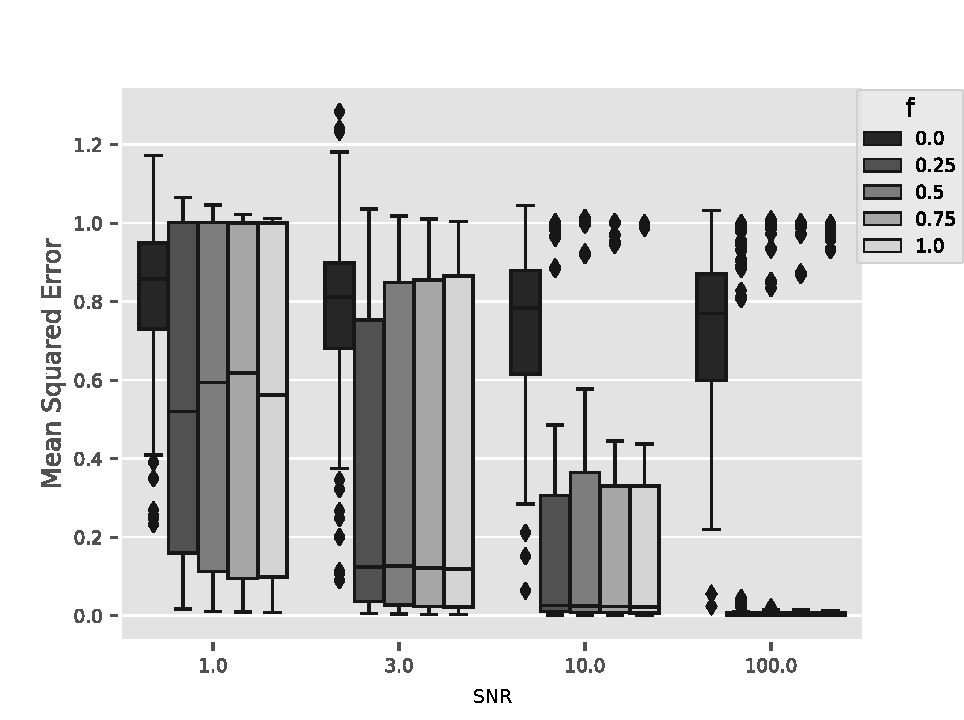
\includegraphics[width=\textwidth]{./tex/fig/mar_pred_err_boxplot.pdf}
        % \caption{Missing at random}
        % \label{fig:synthetic_benchmark_mar_pred_box}
\end{subfigure}%
\caption{
Mean Squared Error of test sets predictions in synthetic datasets.
We show how with already $f \geq 0.25$ (the fraction of observations with all the views) we can significantly reduce the prediction error on testing data-points.
}
\label{fig:synthetic_benchmark_pred_box}
\end{figure}
% \begin{figure}[htb]
% \centering
% \begin{subfigure}{.45\textwidth}
%       \centering
%         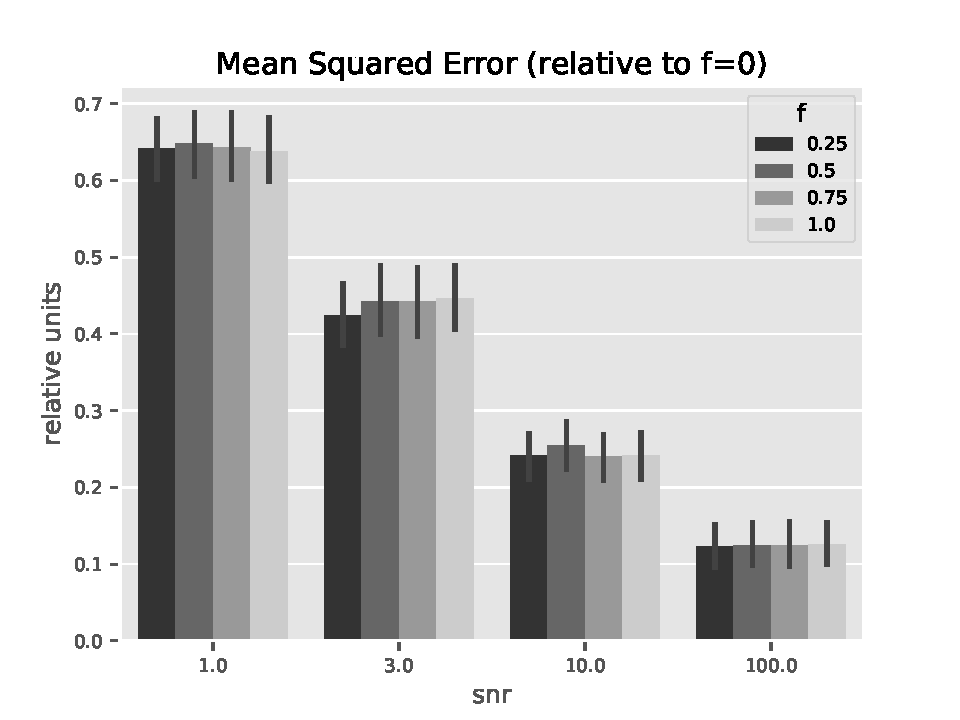
\includegraphics[width=\textwidth]{./tex/fig/mar_barplot.pdf}
%         \caption{Missing at random}
%         \label{fig:synthetic_benchmark_mar_bar}
% \end{subfigure}%
% \hfill
% \begin{subfigure}{.45\textwidth}
%       \centering
%         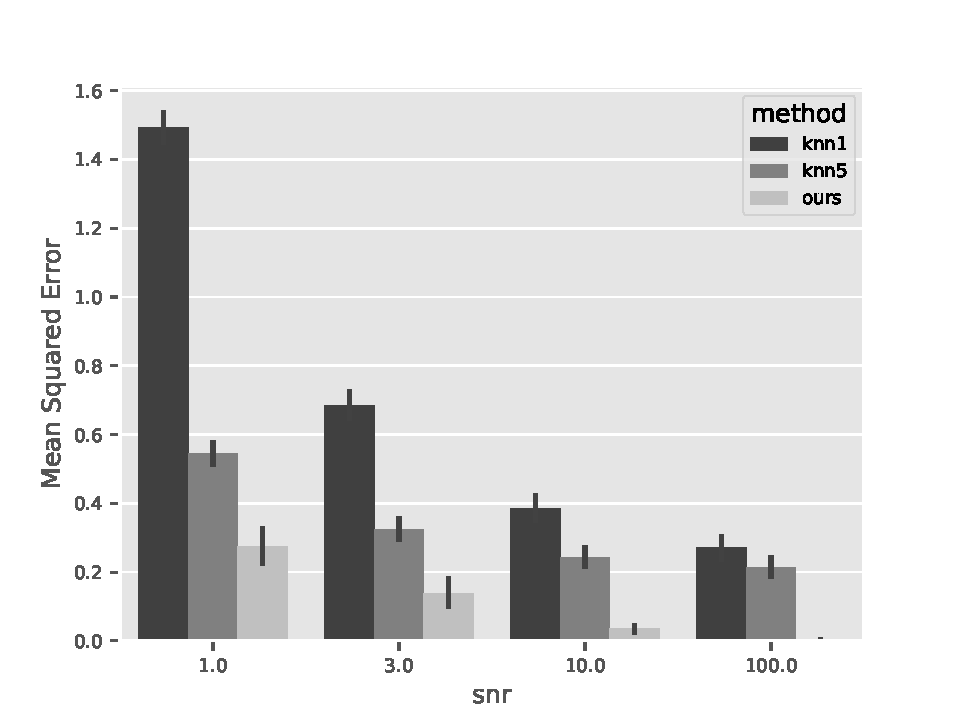
\includegraphics[width=\textwidth]{./tex/fig/mnar_barplot.pdf}
%         \caption{Missing not at random}
%         \label{fig:synthetic_benchmark_mnar_bar}
% \end{subfigure}
% \caption{
% Mean Squared Error of test sets predictions in synthetic datasets. Effect of signal-to-noise ratio (\snr) is shown.
% (a) With $f$ being the fraction of observation with complete views, we show how with already $f \geq 0.25$ we can significantly reduce the prediction error on testing data-points.
% (b) In multi-view datasets where none of the data-point have all the views, and where the available views depends on the specific dataset, we show the prediction performance of our model in comparison with classic k-nearest-neighbors imputation methods.
% }
% \label{fig:synthetic_benchmark_bar}
% \end{figure}



To simulate multi dataset observations, we sample the latent variable $\z_{d,n}$ from a multivariate Gaussian with zero-mean and identity covariance matrix, and then we transform it with random linear mapping towards the observation space to get $\xdnv$.
We then corrupt the observation with increasing levels of noise
and we apply specific strategies to remove views in the context of the \textit{missing at random} (MAR) and \textit{missing not at random} (MNAR) experiments.
%% MAR %%
In the MAR experiments views were randomly removed according to a parameter $0 \leq f \leq 1$ to control the fraction of observation with complete views.
%% MNAR %%
In the MNAR experiments we removed specific views for each simulated dataset, ensuring at the same time the absence of at least one view for a datasets, and the presence of at least one view in common between pairs of datasets.
As an example, in the case with three datasets and three views, the association view-dataset can be expressed through the following association matrix $A$:
\begin{equation}
A = 
\begin{pmatrix}
1 & 0 & 1 \\
1 & 1 & 0 \\
0 & 1 & 1 
\end{pmatrix},
\end{equation}
where $A(v,d)=1$ indicates the presence of view $v$ in dataset $d$.
In both MAR and MNAR experiments we fit the noisy and view-missing observations with our model, where we choose a linear Gaussian parametrization for the variational and likelihood distributions, such that:
\begin{align}
\label{eq:encoder}
q_{d,n,w}(\z) &= \Gaussof{\mub=\mathbf{V}_w^{(\mu)} \xdnw, \Sigmab = diag(\mathbf{V}_w^{(\sigma)} \xdnw)}, \\
\label{eq:decoder}
\p{\xdnv|\z,\thetab_v} &= \Gaussof{\mub = \mathbf{G}_v^{(\mu)} \zb, \Sigmab = diag(\mathbf{g}_v^{(\sigma)})},
\end{align}
\textit{i.e.} factorized multivariate Gaussian distributions whose moments are linear transformations depending on the conditioning variables. \\
$\thetab_v = \{\mathbf{G}_v^{(\mu)}, \mathbf{g}_v^{(\sigma)}\}$ and $\phib_w=\{\mathbf{V}_w^{(\mu)}, \mathbf{V}_w^{(\sigma)}\}$ are the parameters to be optimized through (\ref{eq:argmax}).
Lastly we predicted the missing views according to \eqnref{eq:reconstruction}

\subsubsection{Results}
In both the experimental settings, we apply \eqnref{eq:reconstruction} to predict the missing views.
In the MAR experiments we notice how with already $f \geq 0.25$ we can significantly reduce the prediction error on testing data-points (\figref{fig:synthetic_benchmark_mar_box}).
In the MNAR experiments the benchmark against the standard k-nearest-neighbor ($k \in \set{1,5}$) is favourable towards our model in all conditions (\figref{fig:synthetic_benchmark_mnar_box}).


%%%%%%%%%%%%%%%%%%%%%
%% MEDICAL IMAGING %%
%%%%%%%%%%%%%%%%%%%%%
\subsection{Medical Imaging datasets}
\label{ssec:real}

\begin{table}[!t]
\caption{
Number of subjects per view available in each dataset.
The last columns provide the size of the intersection ($\cap$) and union ($\cup$) of subjects with available views.
The mri from the local dataset is considered as a stand-alone modality as the measures were obtained with a different protocol from the ones in the other datasets.
Notice how in the jont dataset no subject have all the modalities.
}
\centering
\resizebox{\columnwidth}{!}{
\begin{tabular}{lccccc|cc}
\toprule
View:          &  clin &   MRI &  FDG & AV45 &  TAU & $\cap$ & $\cup$ \\
\midrule
Dataset \\
adni1          &   740 &   730 &    - &    - &    - & 730 &  740 \\
adni2          &  1324 &   710 &  424 &  417 &   61 &  53 & 1324 \\
miriad         &    67 &    67 &    - &    - &    - &  67 &   67 \\
oasis3         &   529 &   489 &    - &  148 &    - & 147 &  529 \\
geneva         &   999 &     - &   65 &  120 &   54 &  15 &  999 \\
\midrule
Tot. subjects  &  3659 &  1996 &  489 &  685 &  115 &   0 & 3659 \\
\midrule
Tot. datasets  & 5     & 4     & 2    & 3    & 2    &     &      \\
\bottomrule
\end{tabular}}
\label{table:datasets}
\end{table}

\begin{table}[!t]
\caption{
Mean Squared Error on unseen test data, $5$-fold cross validation.
Mean (standard deviation) across folds are shown. Best results in boldface.
Test data may belong to the same datset used to train the model (within) or on all the other (cross).
Every modality was predicted from the other available ones.
}
\centering
\begin{tabular}{llcccccc}
\toprule
             &       &         clin &          mri &          fdg &         av45 &          tau &   mri local \\
train & test &              &              &              &              &              &              \\
\midrule
adni1 & within &  0.91 (0.11) &  0.95 (0.13) &            - &            - &            - &            - \\
             & cross &  0.91 (0.29) &  1.01 (0.44) &            - &            - &            - &            - \\
\midrule
adni2 & within &  0.77 (0.11) &  \textbf{0.91} (0.20) &  \textbf{0.82} (0.20) &  \textbf{0.93} (0.22) &  1.20 (0.71) &            - \\
             & cross &  0.82 (0.27) &  1.00 (0.41) &            - &  1.28 (0.46) &  1.67 (1.19) &            - \\
\midrule
miriad & within &  0.74 (0.34) &  1.01 (0.52) &            - &            - &            - &            - \\
             & cross &  0.89 (0.15) &  0.99 (0.18) &            - &            - &            - &            - \\
\midrule
local & within &  0.94 (0.28) &            - &            - &  1.20 (0.28) &  1.43 (1.29) &  \textbf{1.23} (0.35) \\
             & cross &  1.29 (0.28) &            - &            - &  1.13 (0.24) &  \textbf{1.17} (0.75) &            - \\
\midrule
\midrule
average & within &  0.84 (0.21) &  0.96 (0.29) &  \textbf{0.82} (0.20) &  1.06 (0.25) &  1.32 (1.00) &  \textbf{1.23} (0.35) \\
        & cross  &  0.98 (0.25) &  1.00 (0.34) &            - &  1.21 (0.35) &  1.42 (0.97) &            - \\
\midrule
\midrule
% all (dae)        & within &  0.56 (0.05) &  1.02 (0.12) &  0.98 (0.24) &  1.02 (0.17) &  1.11 (0.62) &  1.10 (0.34) \\
% all (knn5)        & within &  \textbf{0.65} (0.04) &  1.03 (0.11) &  1.09 (0.20) &  1.42 (0.17) &  1.29 (0.66) &  \textbf{1.23} (0.38) \\
all       & joint &  \textbf{0.65} (0.05) &  0.95 (0.12) &  0.85 (0.21) &  0.99 (0.20) &  \textbf{1.17} (0.64) &  1.25 (0.35) \\
\bottomrule
\end{tabular}
\label{table:crossvalidation_details}
\end{table}

%\begin{table}[!t]
%\caption{
%Same as above, after average-pooling af means and standard deviations by 
%}
%\centering
%\begin{tabular}{lcccccc}
%\toprule
%{} &         clin &          mri &          fdg &         av45 &          tau &   mri local \\
%train/test   &              &              &              &              &              &              \\
%\midrule
%within &  0.84 (0.21) &  0.96 (0.29) &  0.82 (0.20) &  1.06 (0.25) &  1.32 (1.00) &  1.23 (0.35) \\
%cross  &  0.98 (0.25) &  1.00 (0.34) &            - &  1.21 (0.35) &  1.42 (0.97) &            - \\
%joint  &  0.65 (0.05) &  0.95 (0.12) &  0.85 (0.21) &  0.99 (0.20) &  1.17 (0.64) &  1.25 (0.35) \\
%\bottomrule
%\end{tabular}
%\label{table:crossvalidation}
%\end{table}


\begin{table}[!t]
\caption{
Mean Squared Error (MSE) of test data from adni2.
All models were trained on all the available datasets by holding-out data from the adni2 test dataset.
$5$-folds cross validation of MSE is shown as mean (standard deviation).
Best results in boldface are significant with an $\alpha$ level of 0.01 with respect to both competing methods.
}
\centering
\label{tab:model_comparison}
\begin{tabular}{lccc}
\toprule
View       &          \multicolumn{3}{c}{model}\\
           &          dae &         knn5 &           ours        \\ \cline{2-4}
clin       &  0.73 (0.14) &  0.44 (0.05) &          0.45 (0.07) \\
MRI        &  1.23 (0.31) &  0.88 (0.15) &  \textbf{0.70} (0.13) \\
FDG        &  4.20 (0.56) &  4.15 (0.59) &  \textbf{1.09} (0.15) \\
AV45       &  1.45 (0.35) &  1.20 (0.25) &  \textbf{0.89} (0.15) \\
TAU        &  1.54 (0.82) &  1.44 (0.83) &  \textbf{1.05} (0.45) \\
\bottomrule
\end{tabular}
\end{table}

% \begin{table}[!t]
% \caption{
% Add OASIS3 dataset (clin, mri, av45)
% }
% \centering
% \begin{tabular}{lcccccc}
% \toprule
% model &         clin &          mri & fdg &         av45 &          tau & mri local \\
% % model &              &              &     &              &              &            \\
% \midrule
% knn5              &  0.50 (0.06) &  0.92 (0.13) &   - &  \textbf{1.33} (0.23) &  1.10 (0.54) &  -  \\
% dae               &  0.45 (0.08) &  0.95 (0.15) &   - &  1.49 (0.20) &  1.09 (0.50) &  -  \\
% our               &  \textbf{0.39} (0.05) &  \textbf{0.75} (0.13) &   - &  1.38 (0.21) &  \textbf{0.93} (0.51) &  -  \\
% \bottomrule
% \end{tabular}
% \label{table:model_comparison}
% \end{table}
% 
% \begin{table}[!t]
% \caption{
% Add OASIS3 dataset (clin, mri, av45), ComBat normalize (mri, fdg, av45, tau)
% }
% \centering
% \begin{tabular}{lcccccc}
% \toprule
% model &         clin &          mri & fdg &         av45 &          tau & mri local \\
% % model &              &              &     &              &              &            \\
% \midrule
% knn5              &  0.51 (0.07) &  1.10 (0.17) &   - &  1.16 (0.19) &  \textbf{1.08} (0.62) &  -  \\
% dae               &  0.44 (0.06) &  1.09 (0.17) &   - &  \textbf{1.06} (0.19) &  1.45 (0.70) &  -  \\
% our               &  \textbf{0.42} (0.05) &  \textbf{0.94} (0.15) &   - &  \textbf{1.06} (0.20) &  1.32 (0.71) &  -  \\
% \bottomrule
% \end{tabular}
% \label{table:model_comparison}
% \end{table}
% 
% \begin{table}[!t]
% \caption{
% Add OASIS3 dataset (clin, mri, av45), add Geneva PET, ComBat normalize (mri, fdg, av45, tau)
% }
% \centering
% \begin{tabular}{lcccccc}
% \toprule
% model &         clin &          mri & fdg &         av45 &          tau & mri local \\
% % model &              &              &     &              &              &            \\
% \midrule
% knn5              &  0.50 (0.06) &  1.09 (0.17) &   - &  1.18 (0.20)  &  1.23 (0.92)  &  -  \\
% dae               &  0.42 (0.08) &  1.09 (0.16) &   - &  1.08 (0.19)  &  1.54 (0.87)  &  -  \\
% our               &  \textbf{0.41} (0.06) &  \textbf{0.93} (0.15) &   - &  \textbf{1.07} (0.17)  &  \textbf{1.17} (0.81)  &  -  \\
% \bottomrule
% \end{tabular}
% \label{table:model_comparison}
% \end{table}


\subsubsection{Data preparation}
Data used in the preparation of this article were obtained from the following sources.
1) From the Alzheimer's Disease Neuroimaging Initiative (ADNI)
\footnote{
\href{http://adni.loni.usc.edu}{adni.loni.usc.edu}. The ADNI was launched in 2003 as a public-private partnership, led by Principal Investigator Michael W. Weiner, MD. For up-to-date information, see \href{www.adni-info.org}{www.adni-info.org}.
}.
2) From MIRIAD dataset \cite{Miriad}, a database of volumetric MRI brain-scans of Alzheimer's sufferers and healthy elderly people.
3) From a local cohort collected at the University Hospitals, having healthy subjects and subjects with various cognitive disorders.

We divided the ADNI dataset into two independent ones:
`adni1', composed by subjects recruited in the initial study,
and `adni2' composed by those subjects subsequently recruited in ADNI-GO, ADNI2, and ADNI3.
Since data modalities and acquisition protocols of `adni1' are different from those of `adni2', we consider these two cohorts as indipendent datasets.

From the four datasets (`adni1', `adni2', `miriad', `local') we grouped the observations into the following views.
1) `clin': containing age and the Mini-Mental cognitive score (MMSE).
2) `mri': brain volumes computed with FreeSurfer \footnote{
\href{https://surfer.nmr.mgh.harvard.edu/}{surfer.nmr.mgh.harvard.edu}
}.
3) `fdg': average brain glucose uptake measured through the analysis of FDG-PET scans.
4) `av45': average brain amyloid uptake measured through the analysis of AV45-PET scans.
5) `tau': average brain protein Tau uptake measured through the analysis of TAU-PET scans.
6) `mri local': this is a view only present in the `local' dataset, composed by measurements on brain gray matter density derived from SPM \cite{Ashburner2000}.
All the imaging measurements are averaged on the regions of interests defined in the Desikan-Killiany atlas \cite{Desikan2006}
In \tabref{table:datasets} we show the number of observations stratified by dataset and modality.
Please note that the only view in common across datasets is the clinical one, composed by MMSE and age features only.

\subsubsection{Fitting procedure}
For the model architecture, we choose the likelihood function as in \eqnref{eq:decoder}.
We then choose to parametrize the encoder as:
\begin{equation}
\label{eq:dropout_posterior}
    q_{d,n,w}(\z) = \Gauss{\mub = \mathbf{V}_w^{(\mu)} \xdnw}{\Sigmab = \text{diag}(\sqrt{\alphab} \odot \mub)^2}.
\end{equation}
The posterior distribution so defined is known as \textit{dropout posterior}.
The dropout parameter $\alphab$ has components $\alpha_i = \nicefrac{p_i}{1-p_i}$ linked to the probability $p_i$ of dropping out the $i$-th latent variable component \cite{Wang2013}.
It has been shown that the association of this dropout posterior with a log-uniform prior distribution $\pz$ leads to sparse and interpretable models \cite{Antelmi2019,Molchanov2017}.

We fit our multi-view model one dataset at a time, and lastly on the whole dataset pool.
We will refer to this last model as `all'.
Observations were divided into five splits, stratified to keep an intra-dataset proportion of views as close as possible as the ones of the original datasets.
After setting a dropout threshold to $0.5$ we measured, through the mean squared error, the prediction error of the dataset-specific models on the testing hold-out observations of the same dataset (within).
To have a measure of the generalization ability for each model, we measured the prediction accuracy also on all the test sets not belonging to the same dataset of the trainig set (cross).
The same was done with the model `all'.
In this case the hold out observations belong to the whole dataset pool and we will refer to its testing set as the `joint' set.

\subsubsection{Results}
In \tabref{table:crossvalidation_details} we show for each trained multi-view model, the prediction error on the within-dataset test sets, cross-dataset test sets, and joint set, whenever computable.
We notice that the generalization performance of the model `all' is almost always the best in predicting the `clin' and `mri' views.
These are also the views most represented in all the datasets.
We also note that joint model systematically outperforms the dataset-specific models when applyed across dataset.
Moreover it generally provides better predictions even respect to the within-dataset results.
On the other extreme, views belonging only to a specific dataset, such as `fdg' in `adni2' and `mri local' in the `local' dataset are better predicted with dataset-specific models.
In the remainig cases of `av45' and `tau', the joint model seems, on average, to perform better than the single dataset-specific ones.


